\documentclass[../../main]{subfiles}

\renewcommand\thesection{\arabic{section}}


\begin{document}

\section{Multiplexer System} \label{sec:multiplexerSystem}

Now let's focus on the \emph{sensing} part, we will have outputs from different
\emph{sensor modules} and \emph{feedback} from all the \emph{actuators}\footnote{right now
actuator feedback is not implemented.}. So we need a way to gather all these information
for the \esp to process.

The design requirements are:

\begin{itemize}
    \item It should be analog, because we will need to read voltage values.
    \item It should be bi-directional, because the communication to DHT22 sensor\footnote{the
        sensor used for sensing temperature and humidity.} is done via a single pin.
    \item It should have two separately controllable multiplexer units. It would give us
        more flexibility and can be used to communicate with devices that require two
        pins. For example, the ultrasonic sensor \emph{HC-SR04}\footnote{right now we are
        not using the sensor but we need it to measure the reservoir level in the future},
        which requires two pins for communication.
    \item The pins required to operate should be minimum as possible.
\end{itemize}

\subsection{$32$ Bit Multiplexer}

So first of all, we need an \emph{analog multiplexer}. The difference between a \emph{digital
multiplexer} and an \emph{analog multiplexer} is that, the former one generates the output
from the inputs using logic gates, and the latter directly connects\footnote{usually using
\emph{transmission gates}.} the inputs to the output depending on the select lines.

The output of the \emph{digital multiplexer} will be always either be high or low. But in
the case of \emph{analog multiplexer} the output is directly tied to the selected input
through a \emph{transmission gate}. Hence the latter is also \emph{bi-directional} in nature,
and can act as a \emph{demultiplexer}.

\alertNote{
    Also note that the \emph{analog multiplexer} can be used as a \emph{digital multiplexer}.
}

\begin{center}
    {\begin{minipage} [c] {0.55\textwidth}
        For future proofing, let the input count of a single multiplexer set be $32$. That means the
        each set of multiplexer will take a $5$ bit address, and can \emph{read} / \emph{write} to
        $32$ different \emph{source} / \emph{destination}. That would give us the ability to connect
        almost $64$\footnote{given that every sensor uses a single pin to communicate.} different
        \emph{sensors} to the \esp. And can simultaneously use $2$ different \emph{source} / \emph{destination}.

        An ideal candidate for our design is \emph{74HC4067}, which is a $16$ bit
        \emph{analog multiplexer / demultiplexer} with an \emph{active low} enable. Please refer figures
        \ref{fig:74hc4067Smd}, \ref{fig:74hc4067BOB} and \ref{fig:74hc4067PinDiagram} for more information.
        And refer table \ref{tbl:74hc4067RelventPins} for the information about relevant pins.
    \end{minipage}
    \hfill
    \begin{minipage} [c] {0.35\textwidth}
        \centering
        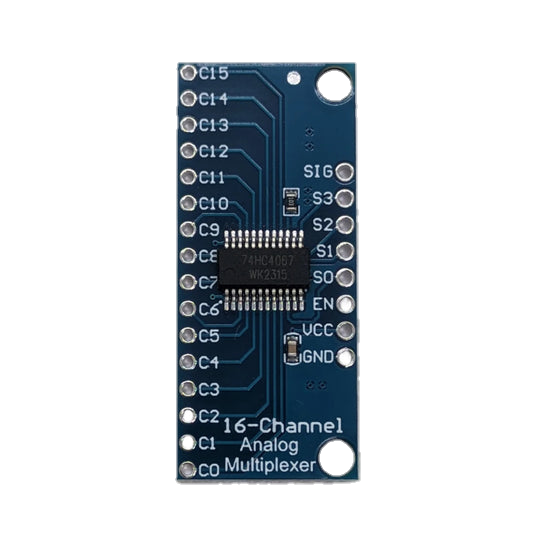
\includegraphics [
            max width = \IGXMaxWidth,
            max height = \IGXMaxHeight,
            \IGXDefaultOptionalArgs,
        ] {pics/74hc4067_bob.png}
        \captionof{figure} {
            Breakout board of \emph{74HC4067}.
            \label{fig:74hc4067BOB}
        }
    \end{minipage}\hfill}
\end{center}

\begin{center}
    {\begin{minipage}[c] {0.42\textwidth}
        \centering

        
\includegraphics [
        ] {pics/74hc4067_smd.pdf}
        \captionof{figure} {
            Smd package of \emph{74HC4067}.
            \label{fig:74hc4067Smd}
        }

        \includegraphics [
            max width = \IGXMaxWidth,
            max height = \IGXMaxHeight,
            \IGXDefaultOptionalArgs,
        ] {tikzpics/endAbsSixteenBitMuxPinout.pdf}
        \captionof{figure} {
            Pin diagram of \emph{74HC4067}.
            \label{fig:74hc4067PinDiagram}
        }

    \end{minipage}
    \begin{minipage}[c] {0.52\textwidth}

        %% TODO: add a description of 74HC4067

        \begin{center}
            \begin{tabularx} {\linewidth} {
                    *{1}{>{\centering\arraybackslash}m{0.5\linewidth}}
                    *{1}{>{\centering\arraybackslash}m{0.5\linewidth}}
                }
                \toprule
                Pins & Remarks \\
                \midrule
                \texttt{C0 - C15} & $16$ channel lines. \\
                \texttt{S0 - S3} & $4$ select lines. \\
                $\overline{\mbox{\texttt{E}}}$ & Enable line. \\
                \texttt{SIG} & Signal line. \\
                \bottomrule
            \end{tabularx}
            \captionof{table} {
                Relevant pins of \emph{74HC4067}.
                \label{tbl:74hc4067RelventPins}
            }
        \end{center}

    \end{minipage}}

\end{center}


\subsection{Serially Addressable Multiplexer}

Now we can simply take two \emph{74HC4067s} and merge them into one $32$ bit multiplexer with
some \emph{home-brew logic gates}. But inorder to drive one of these multiplexers, we need
a total of $7 = 5 (\mbox{address}) + 1 (\mbox{output}) + 1 (\mbox{enable})$ pins. And we would
have $2$ of these in total. That would require a total of $14$ pins from \esp. That's not
feasible.

So we need to find a way to \emph{serially address} the multiplexers. We can simply use a
\emph{shift register} to accomplish our task. \emph{74LS96} is a good candidate for our
scenario, as it is $5$ bit shift register. But choosing \emph{74LS96} has a grave disadvantage,
that is it's a \emph{74LS}\footnote{LS stands for Low-power Schottky.} series IC.
And our multiplexer is \emph{74HC}\footnote{HC stands for High-speed CMOS.} series. The former
belongs to \emph{TTL}\footnote{actually, the LS series uses Schottky transistors, but the
logic voltage levels are comparable to TTL family} logic family and the latter belongs to
\emph{CMOS} logic family. The problem here is that the \emph{CMOS} logic family cannot be driven
by \emph{TTL} logic family. The output high voltage of \emph{74LS} series is too low\footnote{around
$2.2\si{V}$ to $3\si{V}$} for \emph{74HC} series to pick up as a \emph{logic high}.

Inorder to solve this issue, we need to use some \emph{level shifters}. This is where the
\emph{inverters} we have designed in section \ref{sec:bufferOrInverter} comes in play.
Our \emph{74LS96} will drive those \emph{inverters} and they in turn drives the pins of
\emph{74HC4067}.

Choosing \emph{74LS96} has a advantage too, they can be driven by \esp\footnote{output high voltage is
$3.3\si{V}$.} directly as they will take any voltage greater than $2.2\si{V}$ as logic high.

Please refer to figures \ref{fig:74ls96Dip} and \ref{fig:74ls96PinDiagram} for more information about
\emph{74LS96}. And table \ref{tbl:74ls96RelventPins} goes through some pins that are relevant to
our design.

\alertWarning{
    It is wise to tie unused pins, either high or low. In this case the \emph{preset}
    pins of \emph{74LS96} are left floating. They will be read as high by \emph{74LS}
    chips. But if you are using \emph{74HC} or \emph{74HCT} versions of this chip, it
    is recommended to always tie these pins either high or low.
}

\alertImportant{
    Pins $\overline{\mbox{\texttt{E}}}$ and \texttt{PE} of \emph{74LS96} are tied
    \emph{high} and \emph{low} respectively, so as to disable asynchronous resetting
    of the internal latches.
}

\begin{center}
    {\begin{minipage}[c] {0.42\textwidth}
        \centering

        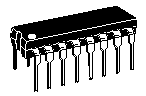
\includegraphics [
        ] {pics/74ls96_dip.pdf}
        \captionof{figure} {
            Dip package of \emph{74LS96}.
            \label{fig:74ls96Dip}
        }

        \includegraphics [
            max width = \IGXMaxWidth,
            max height = \IGXMaxHeight,
            \IGXDefaultOptionalArgs,
        ] {tikzpics/endAbsFiveBitShiftRegisterPinout.pdf}
        \captionof{figure} {
            Pin diagram of \emph{74LS96}.
            \label{fig:74ls96PinDiagram}
        }

    \end{minipage}
    \begin{minipage}[c] {0.52\textwidth}

        \centering

        \begin{tabularx} {\linewidth} {
                *{1}{>{\centering\arraybackslash}m{0.3\linewidth}}
                *{1}{>{\centering\arraybackslash}m{0.7\linewidth}}
            }
            \toprule
            Pins & Remarks \\
            \midrule
            \texttt{PS A - PS E} & Preset lines (We are not using them). \\
            \texttt{Q A - Q E} & Parallel output lines. \\
            $\overline{\mbox{\texttt{MR}}}$ & Master reset (always tied high). \\
            \texttt{PE} & Preset enable (always tied low). \\
            \texttt{CP} & Clock pulse. \\
            \texttt{S} & Serial in. \\
            \bottomrule
        \end{tabularx}
        \captionof{table} {
            Relevant pins of \emph{74LS96}.
            \label{tbl:74ls96RelventPins}
        }

    \end{minipage}}

\end{center}

\subsection{Putting It All Together}

Now that we have sorted out all the components, we can put these all together to make
our \emph{serially addressable $32$ bit multiplexer}. Figure \ref{fig:absThirtyTwoBitMux}
shows the abstract diagram of the internals of our multiplexer.

\begin{figure}
    \centering
    \includegraphics [
        max width = \IGXMaxWidth,
        max height = \IGXMaxHeight,
        \IGXDefaultOptionalArgs,
    ] {tikzpics/endAbsThirtyTwoBitMux.pdf}
    \captionof{figure} {Internals of the $32$ bit multiplexer.}
    \label{fig:absThirtyTwoBitMux}
\end{figure}




\end{document}
